\documentclass[a4paper, 12pt]{article}
\usepackage{geometry}
\geometry{
	a4paper,
	left=30mm,
	top=20mm,
}

\bibliographystyle{apalike}
\usepackage[square, authoryear, comma, sort&compress]{natbib}

\usepackage[english]{babel}
\usepackage[utf8]{inputenc}
\usepackage{amsmath}
\usepackage{amssymb}
\usepackage{amsthm}
\usepackage{mathbbol}
\usepackage{mathtools}
\usepackage{mathrsfs}
\usepackage{graphicx}
\usepackage[colorinlistoftodos]{todonotes}
\usepackage{longtable}
\usepackage{tcolorbox}
\usepackage[colorlinks = true, linkcolor = black, urlcolor  = cyan, citecolor = black, anchorcolor = black]{hyperref}
\usepackage{listings}
\usepackage{wrapfig}
\usepackage{cleveref}
\usepackage{vector}

\lstdefinelanguage{Python}{
	keywords={typeof, null, catch, switch, in, int, str, float, self},
	keywordstyle=\color{ForestGreen}\bfseries,
	ndkeywords={boolean, throw, import},
	ndkeywords={return, class, if ,elif, endif, while, do, else, True, False , catch, def},
	ndkeywordstyle=\color{BrickRed}\bfseries,
	identifierstyle=\color{black},
	sensitive=false,
	comment=[l]{\#},
	morecomment=[s]{/*}{*/},
	commentstyle=\color{purple}\ttfamily,
	stringstyle=\color{red}\ttfamily,
}

\newcommand{\argmax}{\operatornamewithlimits{argmax}}

\title{Multiclass Classification with Kernel Embeddings}

\author{Kelvin Hsu}

\date{\today}

\setlength{\parskip}{1em}

\begin{document}
\maketitle

\section{Motivation}

	Most classification algorithms are binary classifiers, which can only handle the case where the output can only take instances from one of two classes. This is true for both SVM classifiers and GP classifiers. Part of the reason for that is that it works by learning a continuous latent function which basically represents the `strength' of one of the classes, and so it is really just inferring how likely an input is from class A and if not it would be from class B. To build a multiclass classifier, a simple approach is to train multiple binary classifiers to tell apart pairs of classes or sets of classes, and somehow fuse these results together. Notable examples are One Versus All (OVA) and All Versus All (AVA) approaches, as well as binary tree approaches.
	
	\href{http://www.vision.caltech.edu/malaa/publications/aly05multiclass.pdf}{Here} is a 2005 Survey which summarises the state-of-the-art in multiclass classification at the time, which supports what I just said above. It does not seem like the above scenario has fundamentally changed in the past 10+ years, although more sophisticated versions of what was described above has been proposed and tested.
	
\section{Idea}

	The idea I am proposing here is actually very simple and intuitive. Suppose the training data is $\{\bvec{x}_{i}, y_{i}\}_{i = 1}^{n}$ where $\bvec{x}_{i} \in \mathcal{X}, y_{i} \in \mathbb{N}_{m}$ for all $i \in \mathbb{N}_{n}$ with $\mathbb{N}_{m} := \{1, 2, \cdots, m\}$. To clarify, $n$ is the number of training points, $m$ is the number of classes involved, and $\mathcal{X}$ is usually a subset of some euclidean space $\mathbb{R}^{d}$ but it does not necessarily have to be so (which is an advantage in kernel methods in general, such as GPs). The idea is to use the kernel embedding framework to compute a conditional embedding empirically from those training points. We then show that class probabilities can be computed from the conditional embedding if we place a Kronecker delta kernel on the space of the outputs, $\mathbb{N}_{m}$. We show that these class probabilities estimates are consistent estimates of the true class probabilities. Furthermore, the corresponding Shannon information entropy estimate at each query input can be computed, in two different ways, and we explore the performance of each of these approaches. In this way, we propose a natural probabilistic classifier for multiclass classification.
	
	Computationally, this probabilistic classifier is to do the following. Given a set of training points $\{\bvec{x}_{i}, y_{i}\}_{i = 1}^{n}$ and a set of query inputs $\{\bvec{x}^{\star}_{i}\}_{i = 1}^{n^{\star}}$, our classifier can output $\hat{P}^{\star} = \{\hat{\bvec{p}}^{\star}_{i}\}_{i = 1}^{n^{\star}}$, the estimated class probabilities at the query points, and also $\bvec{h}^{\star} = \{\hat{h}^{\star}_{i}\}_{i = 1}^{n^{\star}}$, the estimated information entropy at the query points.
	
\section{Methodology}

	To construct a conditional embedding corresponding to the distribution $\mathbb{P}_{Y | X}$ where $X : \Omega \to \mathcal{X}$ and $Y: \Omega \to \mathcal{Y}$ are measurable random variables, a kernel $k$ for the input space $\mathcal{X}$ and another kernel $l$ for the output space $\mathcal{Y}$ is chosen. They each describe how similarity is measured within each of the respective spaces.
	
	The empirical conditional embedding (I need to cite this) is then given by
	
	\begin{equation}
		\hat{\mu}_{Y | X} = \Psi (K + \lambda I)^{-1} \Phi^{T},
	\end{equation}
	
	where $K := \{k(\bvec{x}_{i}, \bvec{x}_{j})\}_{i = 1, j = 1}^{n, n}$, $\Phi := \begin{bmatrix} k(\bvec{x}_{1}, \cdot) & k(\bvec{x}_{2}, \cdot) & \dots & k(\bvec{x}_{n}, \cdot) \end{bmatrix}$, $\Psi := \begin{bmatrix} l(y_{1}, \cdot) & l(y_{2}, \cdot) & \dots & l(y_{n}, \cdot) \end{bmatrix}$, and $\lambda$ is the regularisation parameter to make sure $C_{X X}$ covers the right range (I will check on the exact technical wording of this but this is not important in the discussion here).
	
	In our context, the output is finite and discrete, taking values only in $\mathcal{Y} = \mathbb{N}_{m}$. Naturally, we choose the Kronecker delta kernel $\delta : \mathbb{N}_{m} \times \mathbb{N}_{m} \to \{0, 1\}$ for the output space, where inputs that are the same has unit similarity and outputs that are different have no similarity. That is, for all $y_{i}, y_{j} \in \mathcal{Y}$,
	
	\begin{equation}
		\delta(y_{i}, y_{j}) = \begin{cases}
			1 & \mathrm{if } \quad y_{i} = y_{j} \\
			0 & \mathrm{otherwise}.
		\end{cases}
	\end{equation}
	
	One can easily check that this is a positive definite kernel and is characteristic.

	Notice that this kernel has no hyperparameters to tune or learn, so that the hyperparameters only come from the kernel of the input space and the regularisation parameter $\lambda$.
	
	Let the reproducing kernel Hilbert space (RKHS) defined by the Kronecker delta kernel be denoted as $\mathcal{H}_{\delta}$.
	
	Recall that the RKHS of a kernel is the closure of the span of the kernel feature basis as follows (from \href{http://www.jmlr.org/papers/volume10/xu09a/xu09a.pdf}{here})
	
	\begin{equation}
		\mathcal{H}_{l} = \overline{\mathrm{span}\{l(y, \cdot) : y \in \mathcal{Y}\}}
	\end{equation}
	
	For $\mathcal{Y} = \mathbb{N}_{m}$, this means that any real-valued function $g$ whose domain is $\mathbb{N}_{m}$ is in the RKHS of $\delta$.
	
	In particular, indicator functions on $\mathbb{N}_{m}$ are in the RKHS, since
	
	\begin{equation}
		\mathbb{1}_{c}(y) = \begin{cases}
			1 & \mathrm{if } \quad y = c \\
			0 & \mathrm{otherwise}.
		\end{cases} = \delta(c, y).
	\end{equation}
	
	That is, indicator functions $\mathbb{1}_{c} = \delta(c, \cdot)$ for all $c \in \mathbb{N}_{m}$ are simply the canonical kernel features of the RKHS.
	
	We know that the expectation of a function in the RKHS can be written as the inner product of the conditional embedding and the function. When the true conditional embedding is not available, the expectation can be approximated by the inner product of the empirical conditional embedding and the function (I need to cite this, and look up the convergence rate). That is,
	
	\begin{equation}
		\mathbb{E}[g(Y) | \bvec{X} = \bvec{x}^{\star}] = \langle \mu_{Y | \bvec{X} = \bvec{x}^{\star}}, g \rangle \approx \langle \hat{\mu}_{Y | \bvec{X} = \bvec{x}^{\star}}, g \rangle.
	\end{equation}
	
	for all $g \in \mathcal{H}_{l}$.
	
	So, for our case of $\mathcal{H}_{\delta}$ being the RKHS corresponding to the output space, since $\mathbb{1}_{c} \in \mathcal{H}_{\delta}$, we have
	
	\begin{equation}
		p^{\star}_{c} := \mathbb{P}[Y = c | \bvec{X} = \bvec{x}^{\star}] = \mathbb{E}[\mathbb{1}_{c}(Y) | \bvec{X} = \bvec{x}^{\star}] = \langle \mu_{Y | \bvec{X} = \bvec{x}^{\star}}, \mathbb{1}_{c}  \rangle \approx \langle \hat{\mu}_{Y | \bvec{X} = \bvec{x}^{\star}}, \mathbb{1}_{c}  \rangle.
	\end{equation}	

	Note that all quantities are conditioned on the training set and thus is dropped from the notation. This is in turn equal to the following,
	
	\begin{equation}
		\begin{aligned}
			& \langle \hat{\mu}_{Y | X = x}, \mathbb{1}_{c}  \rangle \\
			= & \mathbb{1}_{c}^{T} \Psi (K + \lambda I)^{-1} \Phi^{T} k(\bvec{x}^{\star}, \cdot) \\
			= & \mathbb{1}_{c}^{T} \begin{bmatrix} l(y_{1}, \cdot) & l(y_{2}, \cdot) & \dots & l(y_{n}, \cdot) \end{bmatrix} (K + \lambda I)^{-1} \begin{bmatrix} k(\bvec{x}_{1}, \cdot)^{T} \\ k(\bvec{x}_{2}, \cdot)^{T} \\ \vdots \\ k(\bvec{x}_{n}, \cdot)^{T} \end{bmatrix} k(\bvec{x}^{\star}, \cdot) \\
			= & \begin{bmatrix} \mathbb{1}_{c}^{T}l(y_{1}, \cdot) & \mathbb{1}_{c}^{T}l(y_{2}, \cdot) & \dots & \mathbb{1}_{c}^{T}l(y_{n}, \cdot) \end{bmatrix} (K + \lambda I)^{-1} \begin{bmatrix} k(\bvec{x}_{1}, \cdot)^{T} k(\bvec{x}^{\star}, \cdot) \\ k(\bvec{x}_{2}, \cdot)^{T} k(\bvec{x}^{\star}, \cdot)\\ \vdots \\ k(\bvec{x}^{\star}_{n}, \cdot)^{T} k(\bvec{x}^{\star}, \cdot) \end{bmatrix} \\
			= & \begin{bmatrix} \mathbb{1}_{c}(y_{1}) & \mathbb{1}_{c}(y_{2}) & \dots & \mathbb{1}_{c}(y_{n}) \end{bmatrix} (K + \lambda I)^{-1} \begin{bmatrix} k(\bvec{x}_{1}, \bvec{x}^{\star}) \\ k(\bvec{x}_{2}, \bvec{x}^{\star}) \\ \vdots \\ k(\bvec{x}_{n}, \bvec{x}^{\star}) \end{bmatrix} \\
			= & \bvec{1}_{c}^{T} (K + \lambda I)^{-1} \bvec{k}_{\bvec{x}^{\star}},
		\end{aligned}
	\end{equation}
	
	where $\bvec{1}_{c} := \{\mathbb{1}_{c}(y_{i})\}_{i = 1}^{n}$ and $\bvec{k}_{\bvec{x}^{\star}} := \{k(\bvec{x}_{i}, \bvec{x}^{\star})\}_{i = 1}^{n}$.
	
	Hence, our main result is
	
	\begin{equation}
		\hat{p}^{\star}_{c} = \bvec{1}_{c}^{T} (K + \lambda I)^{-1} \bvec{k}_{\bvec{x}^{\star}}.
	\label{eq:probabilities}
	\end{equation}
	
	Computationally, this can also be vectorised over multiple classes as
	
	\begin{equation}
		\hat{\bvec{p}}^{\star} = B^{T} (K + \lambda I)^{-1} \bvec{k}_{\bvec{x}^{\star}} \in \mathbb{R}^{m},
	\end{equation}
	
	where $B = \begin{bmatrix} \bvec{1}_{1} & \bvec{1}_{2} & \cdots & \bvec{1}_{m} \end{bmatrix} \in \{0, 1\}^{n \times m}$. I choose $B$ as the notation to stand for binary, since the matrix can only take on values of $0$s and $1$s.
	
	It can further be vectorised over multiple query points $\{\bvec{x}^{\star}_{i}\}_{i = 1}^{n^{\star}}$ as usual through
	
	\begin{equation}
		\hat{P}^{\star} = B^{T} (K + \lambda I)^{-1} K^{\star} \in \mathbb{R}^{m},
	\end{equation}
	
	where $K^{\star} = \{k(\bvec{x}_{i}, \bvec{x}_{j}^{\star})\}_{i = 1, j = 1}^{n, n^{\star}}$.
	
	Of course, this is only an estimate, which will converge to the true probabilities as $n$ increases due to the convergence properties of kernel embeddings (cite this). As such, it does not necessarily sum up to one, nor does it necessarily have to be within the range $[0, 1]$, although it will be very close to it.
	
	For prediction, this is not a problem, as for each query point $\bvec{x}^{\star}$ we simply taken the class that has the highest estimated probability to be the prediction. That is, at the query point $\bvec{x}^{\star}$ the prediction is
	
	\begin{equation}
		\hat{y}^{\star} = \argmax_{c \in \mathbb{N}_{m}} \hat{p}_{c}^{\star}.
	\end{equation}
	
	If proper probabilities are required for interpretation, visualisation, or other purposes, the probabilities can be clip normalised as follows,
	
	\begin{equation}
		\tilde{p}^{\star}_{c} := \frac{\max\{\hat{p}^{\star}_{c}, 0\}}{\sum_{j = 1}^{m} \max\{\hat{p}^{\star}_{j}, 0\}}.
	\end{equation}
	
	Experiments verify the fact that clip normalisation does not alter the probabilities by that much, merely making sure they are valid probabilities by slight scaling.
	
	\subsection{Entropy}
	
		The information entropy of our predictions can also be computed. This is ideal for detecting the decision boundaries of the classifier and quantifying how uncertain the prediction is.
		
		There are two ways the information entropy can be approximated or computed. The first way is straight forward, which involves simply computing the information entropy with the clip normalised probabilities, at each query point,
		
		\begin{equation}
			\tilde{h}^{\star} := - \sum_{c = 1}^{m} \tilde{p}^{\star}_{c} \log{\tilde{p}^{\star}_{c}}.
		\end{equation}
		
		The second and more principled way is to also express the entropy as an inner product of an RKHS function with the conditional embedding.
		
		The entropy of the prediction at an output is
		
		\begin{equation}
			\begin{aligned}
				\mathbb{H}[Y | \bvec{X} = \bvec{x}^{\star}] &= - \sum_{c = 1}^{m} \mathbb{P}[Y = c| \bvec{X} = \bvec{x}^{\star}] \log{\mathbb{P}[Y = c | \bvec{X} = \bvec{x}^{\star}]} \\
				&= \mathbb{E}[- \log{\mathbb{P}[Y | \bvec{X} = \bvec{x}^{\star}]} | \bvec{X} = \bvec{x}^{\star}] \\
				&= \mathbb{E}[g(Y) | \bvec{X} = \bvec{x}^{\star}],
			\end{aligned}
		\end{equation}
		
		where 
		
		\begin{equation}
			g(y) := - \log{\mathbb{P}[Y = y | \bvec{X} = \bvec{x}^{\star}]}.
		\end{equation}
		
		If $g$ is in the RKHS $\mathcal{H}_{\delta}$, then we know that this expectation can also be approximated by the inner product of the empirical conditional embedding and the function.
		
		Now we can write $g$ in the following manner
		
		\begin{equation}
			g(y) = \sum_{c = 1}^{m} - \log{\mathbb{P}[Y = c | \bvec{X} = \bvec{x}^{\star}]} \delta(c, y).
		\end{equation}
		
		This shows that $g$ is in the span of the kernel feature and is thus in the RKHS.
		
		Hence, similar to the case with the prediction probabilities, we can write
		
		\begin{equation}
			\mathbb{H}[Y | \bvec{X} = \bvec{x}^{\star}] = \langle \mu_{Y | \bvec{X} = \bvec{x}^{\star}}, g \rangle \approx \langle \hat{\mu}_{Y | \bvec{X} = \bvec{x}^{\star}}, g \rangle.
		\end{equation}
		
		Similar to before the approximation can be written as
		
		\begin{equation}
			\langle \hat{\mu}_{Y | \bvec{X} = \bvec{x}^{\star}}, g \rangle = \bvec{g}^{T} (K + \lambda I)^{-1} \bvec{k}_{\bvec{x}^{\star}},
		\end{equation}
		
		where $\bvec{g} := \{g(y_{i})\}_{i = 1}^{n}$.
		
		Unfortunately, $g$ is not known exactly, since $\mathbb{P}[Y = c | \bvec{X} = \bvec{x}^{\star}]$ is not known exactly. Instead, we consider the approximation $\hat{g}$ of this function $g$ using \eqref{eq:probabilities},
		
		\begin{equation}
			\hat{g}(y) := - \log{\hat{p}^{\star}_{y}} U(\hat{p}^{\star}_{y}),
		\end{equation}
		
		where $U$ is the heaviside function to avoid contributions from negative values.

		We then approximate the entropy with 
		
		\begin{equation}
			\mathbb{H}[Y | \bvec{X} = \bvec{x}^{\star}] \approx \langle \hat{\mu}_{Y | \bvec{X} = \bvec{x}^{\star}}, \hat{g} \rangle = \hat{\bvec{g}}^{T} (K + \lambda I)^{-1} \bvec{k}_{\bvec{x}^{\star}},
		\end{equation}
		
		where $\hat{\bvec{g}} := \{\hat{g}(y_{i})\}_{i = 1}^{n}$.
		
		Again, the information entropy here can be negative, as an artefact of the approximation. We then show that this converges to the actual entropy as $n$ increases (need to do this).

\section{Discussion}

	TALK ABOUT HYPERPARAMETER LEARNING
	
	TALK ABOUT USING BAYESIAN LEARNING OF HYPERPARAMETERS FOR THE INPUT SPACE AND WHY IT STILL MAY NOT BE IDEAL
		
	\subsection{Results}
	
		The results below is obtained through training under a 10-fold cross validation scheme. The kernel used is Gaussian with a sensitivity and a length scale parameter. The regularisation parameter was also trained. Hence, a total of three hyperparameters are used in the model and all of them are trained.

		\begin{figure}[!htbp]
			\centering
			\includegraphics[width=0.8\linewidth]{figures/10cv/figure1.eps}
			\caption{Kernel Embedding Classifier Results: 10-fold cross validation}
			\label{fig:figure_1}
		\end{figure}
		
		\begin{figure}[!htbp]
			\centering
			\includegraphics[width=0.8\linewidth]{figures/10cv/figure2.eps}
			\caption{Kernel Embedding Classifier Results: 10-fold cross validation}
			\label{fig:figure_2}
		\end{figure}
		
		\begin{figure}[!htbp]
			\centering
			\includegraphics[width=0.8\linewidth]{figures/10cv/figure3.eps}
			\caption{Kernel Embedding Classifier Results: 10-fold cross validation}
			\label{fig:figure_3}
		\end{figure}
		
		\begin{figure}[!htbp]
			\centering
			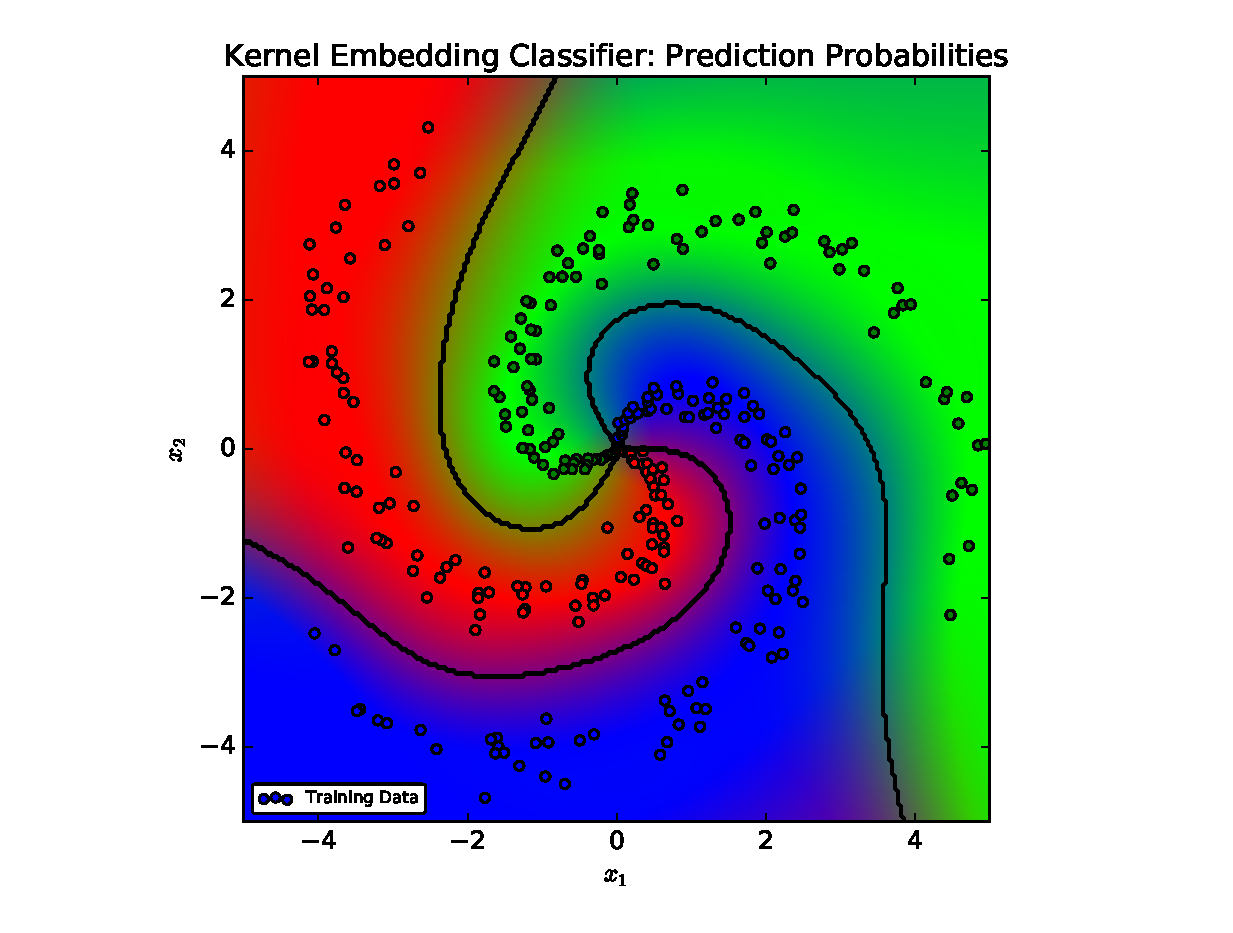
\includegraphics[width=0.8\linewidth]{figures/10cv/figure4.eps}
			\caption{Kernel Embedding Classifier Results: 10-fold cross validation}
			\label{fig:figure_4}
		\end{figure}
		
		\newpage
		WHY CROSS-VAL IS NOT IDEAL
		
		Well, as you can see below, I used 5-fold cross validation and the results are vastly different. Not to mention if I kept it at 10-folds but split the folds differently I would also get slightly different results.
		
		The next step is to try to figure out how to train this classifier without cross validation, hopefully under a Bayesian learning scheme.

		\begin{figure}[!htbp]
			\centering
			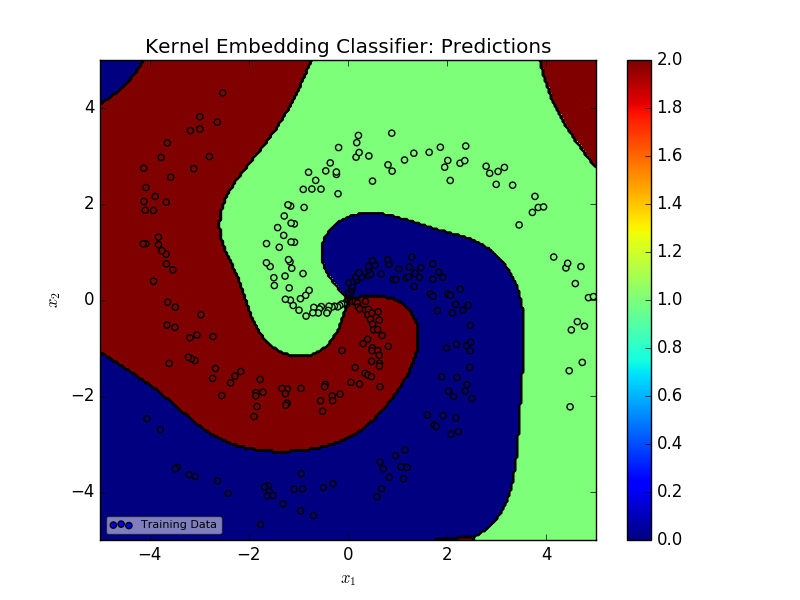
\includegraphics[width=0.8\linewidth]{figures/5cv/figure_1.png}
			\caption{Kernel Embedding Classifier Results: 5-fold cross validation}
			\label{fig:5figure_1}
		\end{figure}
		
		\begin{figure}[!htbp]
			\centering
			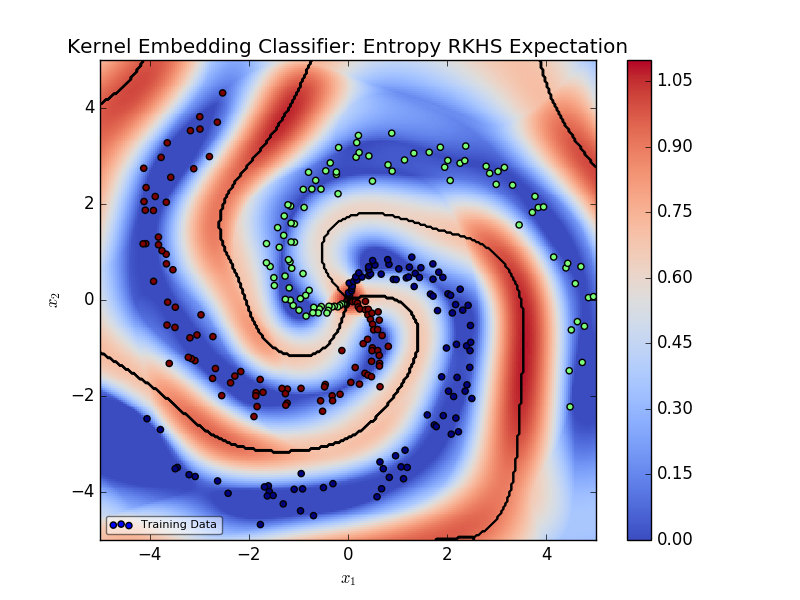
\includegraphics[width=0.8\linewidth]{figures/5cv/figure_2.png}
			\caption{Kernel Embedding Classifier Results: 5-fold cross validation}
			\label{fig:5figure_2}
		\end{figure}
		
		\begin{figure}[!htbp]
			\centering
			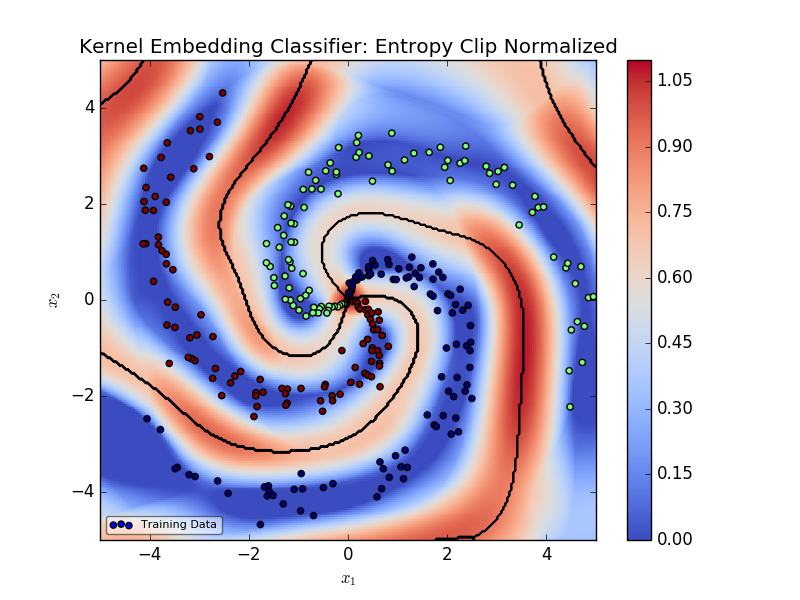
\includegraphics[width=0.8\linewidth]{figures/5cv/figure_3.png}
			\caption{Kernel Embedding Classifier Results: 5-fold cross validation}
			\label{fig:5figure_3}
		\end{figure}
		
		\begin{figure}[!htbp]
			\centering
			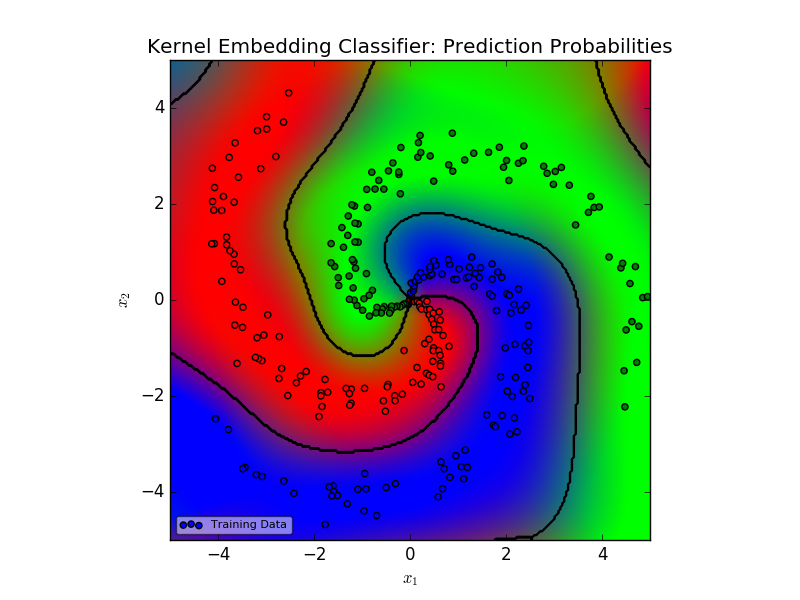
\includegraphics[width=0.8\linewidth]{figures/5cv/figure_4.png}
			\caption{Kernel Embedding Classifier Results: 5-fold cross validation}
			\label{fig:5figure_4}
		\end{figure}
		
	\newpage
	\subsection{Comparisons}

		On the other hand, this is what support vector machines spit out (using sklearn).
		
		Empirically, they are very similar, with similar performances (both 99.3\% accuracy so far).
		
		However, theoretically the kernel embedding classifier is much nicer. For support vector classifiers, the multi-class classifier is built from multiple binary classifiers, whereas the kernel embedding classifier works the same way no matter how many classes there are and handles it very naturally. For the support vector classifier, the probabilities are computed in a very roundabout way, unlike the kernel embedding formulation (check out the 2004 paper by Ting-Fan Wu for how those probabilities in SVMs are calculated). In some sense, both the probabilities and entropy from the SVM are a bit artificial, where as the kernel embedding classifier deals with probability distributions naturally.
		

		\begin{figure}[!htbp]
			\centering
			\includegraphics[width=0.8\linewidth]{figures/10cv/figure5.eps}
			\caption{Support Vector Classifier Results}
			\label{fig:figure_5}
		\end{figure}
		
		\begin{figure}[!htbp]
			\centering
			\includegraphics[width=0.8\linewidth]{figures/10cv/figure6.eps}
			\caption{Support Vector Classifier Results}
			\label{fig:figure_6}
		\end{figure}
		
		\begin{figure}[!htbp]
			\centering
			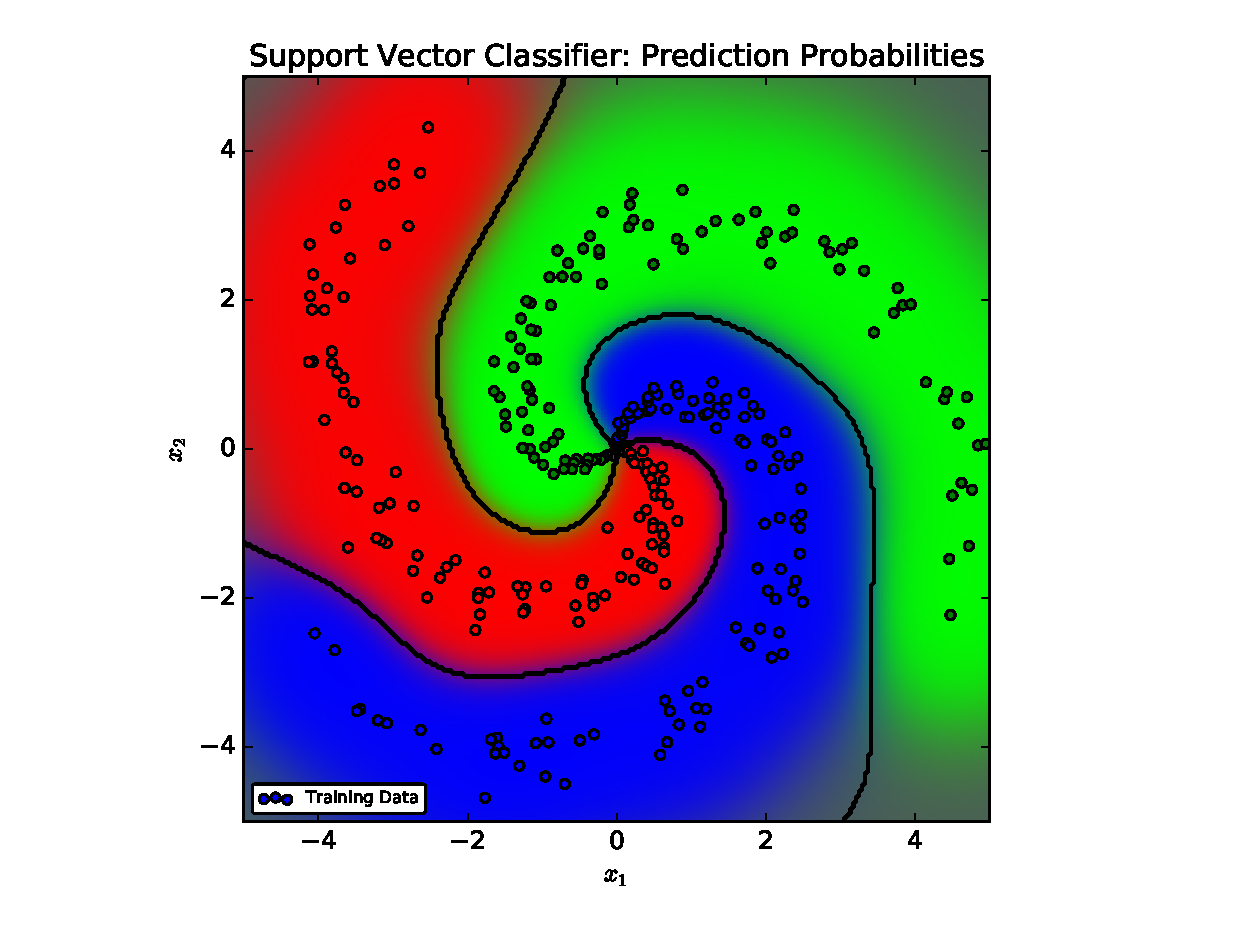
\includegraphics[width=0.8\linewidth]{figures/10cv/figure7.eps}
			\caption{Support Vector Classifier Results}
			\label{fig:figure_7}
		\end{figure}
		
%\bibliography{}

\end{document}